\section{Experiment Results}
\label{section-results}


\subsection{Experimental Setup}

We mainly study three LLMs: GPT-4o, Llama 3.1 70B Instruct, and Llama 3.1 8B Instruct\footnote{More results on five additional LLMs are reported in \Cref{appendix-more-llm-results}.}. For the retriever, we choose dense retrieval with the 1.5B Stella V5 model \citep{zhang_stella_en_1.5B_v5}, given its high performance on MTEB \citep{muennighoff-etal-2023-mteb}. Extensive comparisons between Stella V5 and alternative retrievers are provided in \Cref{appendix-retriever}. For the indexing stage, we employ Llama 3.1 8B Instruct to extract summaries, keyphrases, user facts, and timestamped events. When sessions or rounds are used as the key, we only keep the user-side utterances. In the reading stage, the retrieved items are always sorted by their timestamp to help the reader model maintain temporal consistency. Throughout \Cref{section-value-results} to \Cref{section-query-results}, we apply Chain-of-Note and json format (discussed in \Cref{section-reading-results}) by default. %All experiments were conducted on a local server with 8 NVIDIA A6000 GPUs.


 \begin{figure}[t]
 \centering
 % \vspace{-4mm}
 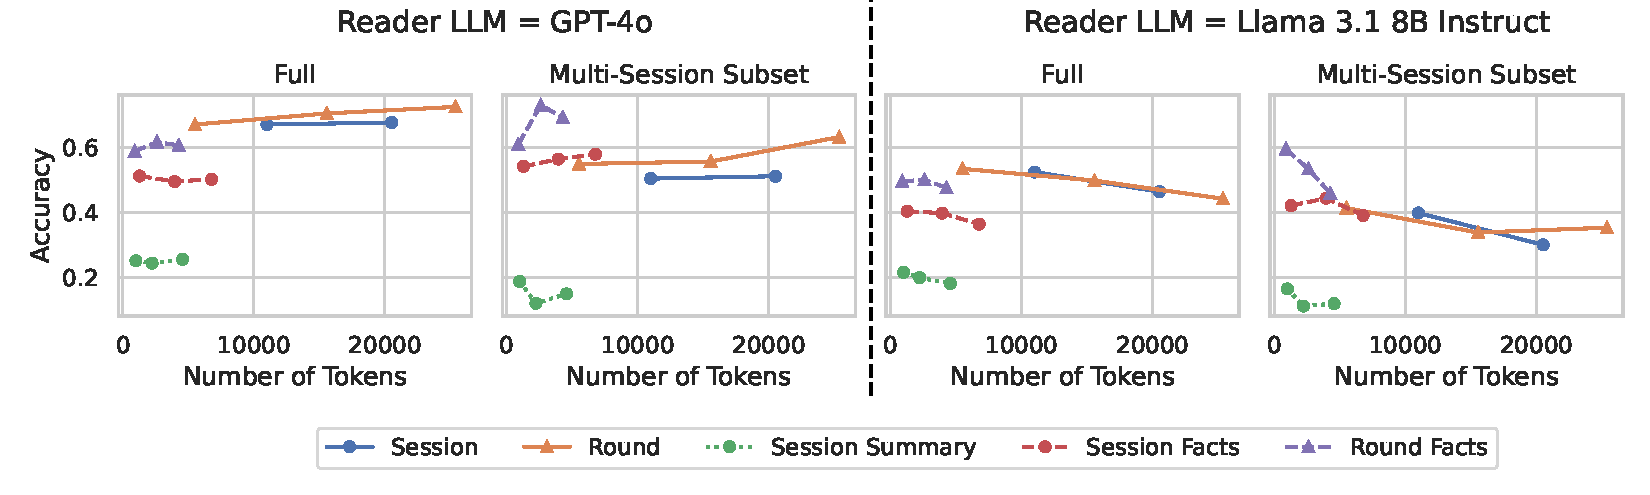
\includegraphics[width=0.95\textwidth]{figures/value_main_500sess.pdf} 
 \vspace{-2mm}
 \caption{QA performance on \BENCHMARK\textsubscript{\textsc{M}} with different value designs. Decomposing sessions into rounds improves the QA performance. For the multi-session reasoning questions, further representing the values with the extracted facts improves the QA accuracy.}
 \vspace{-5mm}
 \label{fig:main-fig-value-design}
\end{figure}

\subsection{Value: Decomposition improves RAG performance}
\label{section-value-results}


Using \BENCHMARK\textsubscript{\textsc{M}}, we compare different value choices in a budget-aware manner. As shown in \Cref{fig:main-fig-value-design}, decomposing sessions into rounds significantly enhances reading performance with GPT-4o as the reader, while performing similarly to non-decomposed sessions when using Llama 3.1 8B Instruct as the reader. However, despite their efficiency in token usage, replacing sessions or rounds with extracted summaries or facts negatively impacts QA performance due to information loss. The only exception is with multi-session reasoning questions, where fact decomposition consistently improves performance. We hypothesize this is because fact decomposition extracts the same type of information across all sessions in a more uniform and simplified format, aiding retrieval and reading \citep{DBLP:journals/corr/abs-2312-06648}. Finally, we observe that the optimal token budget varies by the reader's capability: while Llama 3.1 8B Instruct's performance drops sharply beyond 3k retrieved tokens, GPT-4o continues to improve even with over 20k retrieved tokens.



\subsection{Key: Multi-key indexing improves retrieval and RAG}
\label{section-key-results}

In \Cref{tab:main-results-key}, we explore whether summaries, keyphrases, or user facts condensed from the value can serve as better keys than the value itself. Interestingly, despite their more focused semantics, using these condensed forms alone does not enhance the memory recall performance. We hypothesize that this is due to the retriever's ability to already effectively handle long-text semantics. 


To leverage both the highlighted information from compression and the completeness of the original value, we applied a simple document expansion technique \citep{tao-etal-2006-language, DBLP:conf/sigir/EfronOF12}, where the compressed information is concatenated with the original value to form the key during indexing\footnote{We also experimented with merging at the retrieval stage by combining the ranks from different pathways, but it underperformed compared to indexing-stage merging. See \Cref{appendix-rank-merging} for details.}. This approach, particularly when using user facts, {yielded an average improvement of 9.4\% in recall@$k$ and 5.4\% in final accuracy across all models.} In \Cref{appendix-retriever}, we further analyze different retrievers and find with alternative retrievers, key expansion with summary and keyphrases could improve Recall@5 when session is used as the value granularity. These results suggest that multi-pathway retrieval can significantly enhance memory recall performance. In the following section, we will investigate the time constraint as another pathway to leverage.



 \setlength{\tabcolsep}{3.5pt}
\begin{table}[t]
\centering
\caption{Retrieval and end-to-end QA performance on \BENCHMARK\textsubscript{\textsc{M}} with different key designs for indexing. L3.1 = Llama 3.1 Instruct. We find applying document expansion with the extracted user facts (row K = V + fact) greatly improves both retrieval and the downstream QA.}
\resizebox{0.9\linewidth}{!}{
\renewcommand{\arraystretch}{1.2}
\begin{tabular}{l|cc cc | cc  cc  cc}
\hline
\multirow{4}{*}{\textbf{Key Design}} & \multicolumn{4}{c|}{\textbf{Retrieval}} & \multicolumn{6}{c}{\textbf{End-to-End QA}} \\
\cmidrule(lr){2-5} \cmidrule(lr){6-11}
 & \multicolumn{2}{c}{\textbf{Metrics@5}}  & \multicolumn{2}{c|}{\textbf{Metrics@10}} & \multicolumn{2}{c}{\textbf{GPT-4o}} & \multicolumn{2}{c}{\textbf{L3.1 70B}} & \multicolumn{2}{c}{\textbf{L3.1 8B}} \\
 & \textbf{Recall} & \textbf{NDCG} & \textbf{Recall} & \textbf{NDCG} & \textbf{Top-5} & \textbf{Top-10} & \textbf{Top-5} & \textbf{Top-10} & \textbf{Top-5} & \textbf{Top-10} \\ 
 \hline
\rowcolor{gray!20} \multicolumn{11}{c}{\textbf{Value = Round}} \\
\hline
K = V & 0.582 & 0.481 & 0.692 & 0.512 & 0.615 & 0.670 & 0.600 & 0.624 & 0.518 & 0.534 \\
\hdashline
K = fact & 0.530 & 0.411 & 0.654 & 0.449 & 0.588 & 0.664 & 0.564 & 0.610 & 0.510 & 0.534 \\
K = keyphrase & 0.282 & 0.159 & 0.392 & 0.303 & 0.425 & 0.489 & 0.404 & 0.450 & 0.378 & 0.432 \\
\hdashline
K = V + fact  & \textbf{0.644} & \textbf{0.498} & \textbf{0.784} & \textbf{0.536} & \textbf{0.657} & \textbf{0.720} & \textbf{0.638} & \textbf{0.682} & \textbf{0.566} & \textbf{0.572} \\
K = V + keyphrase  & 0.478 & 0.359 & 0.636 & 0.410 & 0.541 & 0.652 & 0.538 & 0.620 & 0.472 & 0.524 \\
\hline
\rowcolor{gray!20} \multicolumn{11}{c}{\textbf{Value = Session}} \\
\hline
K = V & 0.706 & 0.617 & 0.783 & 0.638 & 0.670 & 0.676 & 0.592 & 0.570 & 0.524 & 0.464 \\
\hdashline
K = summary & 0.572 & 0.448 & 0.648 & 0.468 & 0.554 & 0.252 & 0.498 & 0.512 & 0.444 & 0.216 \\
K = fact & 0.642 & 0.524 & 0.814 & 0.571 & 0.644 & 0.512 & 0.544 & 0.550 & 0.470 & 0.404 \\
K = keyphrase & 0.482 & 0.375 & 0.576 & 0.401 & 0.618 & 0.498 & 0.440 & 0.450 & 0.388 & 0.414 \\
\hdashline
K = V + summary  & 0.689 & 0.608 & 0.749 & 0.624 & 0.658 & 0.666 & 0.568 & 0.560 & 0.518 & 0.494 \\
K = V + fact  & \textbf{0.732} & \textbf{0.620} & \textbf{0.862} & \textbf{0.652} & \textbf{0.714} & \textbf{0.700} & 0.588 & \textbf{0.584} & \textbf{0.530} & 0.490 \\
K = V + keyphrase  & 0.710 & 0.587 & 0.768 & 0.602 & 0.665 & 0.672 & \textbf{0.590} & 0.566 & 0.526 & \textbf{0.508} \\
\hline
\end{tabular}
}
\vspace{-4mm}
\label{tab:main-results-key}
\end{table}


 
\subsection{Query: Time-aware query expansion improves temporal reasoning}
\label{section-query-results}


A key challenge highlighted by \BENCHMARK{} in building real-world assistant systems is the need to utilize temporal information present in both metadata and user utterances to correctly answer time-sensitive queries. To address this need, we introduce a simple yet effective \textit{time-aware indexing and query expansion} scheme. Specifically, values are additionally indexed by the dates of the events they contain. During retrieval, an LLM $\mathcal{M}_{T}$ extracts a time range for time-sensitive queries, which is used to filter out a large number of irrelevant values.

As shown in \Cref{tab:temp-query-results}, {this simple design improves recall by an average of 11.3\% when using rounds as the value and by 6.8\% when using sessions as the value.} This improvement remains consistent when key expansion is applied during indexing. We also find that the effectiveness of this method depends on using a strong LLM for $\mathcal{M}_{T}$ to accurately infer time ranges from queries. Llama 8B, on the other hand, struggles to generate accurate time ranges, often hallucinating or missing temporal cues even with numerous in-context examples. Further analysis is provided in \Cref{appendix-temp-expansion-analysis}.



 % \begin{table}[t]{
%   \centering
%   \caption{Retrieval performance on the temporal reasoning subset of \BENCHMARK\textsubscript{\textsc{M}}. Time-aware query expansion significantly facilitates retrieval by narrowing down the retrieval scope.}
%   \resizebox{\textwidth}{!}{%
%   \begin{tabular}{l|cccc |cccc}
%     \toprule
%     \multirow{3}{*}{\textbf{Key Setting}} & \multicolumn{4}{c}{\textbf{Value = Session}} & \multicolumn{4}{c}{\textbf{Value = Round}} \\
%     \cmidrule(lr){2-5} \cmidrule(lr){6-9}
%      & \multicolumn{2}{c}{Metric@5} & \multicolumn{2}{c}{Metric@10} & \multicolumn{2}{c}{Metric@5} & \multicolumn{2}{c}{Metric@10} \\
%     \cmidrule(lr){2-3} \cmidrule(lr){4-5} \cmidrule(lr){6-7} \cmidrule(lr){8-9}
%      & Recall & NDCG & Recall & NDCG & Recall & NDCG & Recall & NDCG \\
%     \midrule
%     (1) K = V & 0.639 & 0.630 & 0.651 & 0.707 & 0.421 & 0.462 & 0.499 & 0.511 \\
%     (1) w/ Query Expansion ($\mathcal{M}_{T}$ = GPT-4o) & 0.654 & 0.660 & 0.707 & 0.679 & 0.451 & 0.565 & 0.495 & 0.538 \\
%     (1) w/ Query Expansion ($\mathcal{M}_{T}$ = Llama 3.1 8B Instruct) & 0.624 & 0.627 & 0.647 & 0.692 & 0.384 & 0.448 & 0.489 & 0.488 \\
%     \hdashline
%     (2) K = V + fact  & 0.684 & 0.688 & 0.721 & \textbf{0.782} & 0.489 & 0.500 & 0.550 & 0.598 \\
%     (2) w/ Query Expansion ($\mathcal{M}_{T}$ = GPT-4o) & \textbf{0.722} & \textbf{0.732} & \textbf{0.797} & 0.758 & \textbf{0.526} & \textbf{0.548} & \textbf{0.722} & \textbf{0.669} \\
%     (2) w/ Query Expansion ($\mathcal{M}_{T}$ = Llama 3.1 8B Instruct) & 0.677 & 0.688 & 0.711 & 0.744 & 0.481 & 0.532 & 0.570 & 0.647 \\
%     \bottomrule
%   \end{tabular}}
%   \label{tab:temp-query-results}
%   \vspace{-3mm}
%   }
% \end{table}


\begin{table}[t]{
% \vspace{-2mm}
  \centering
  \caption{Retrieval performance on the temporal reasoning subset of \BENCHMARK\textsubscript{\textsc{M}}. Time-aware query expansion significantly facilitates retrieval by narrowing down the retrieval scope.}
  \vspace{-2mm}
  \resizebox{0.97\textwidth}{!}{%
  \begin{tabular}{l|c c c c|c c c c}
    % \hline
    \toprule
    \multirow{3}{*}{\textbf{Key Setting}} & \multicolumn{4}{c|}{\textbf{Value = Session}} & \multicolumn{4}{c}{\textbf{Value = Round}} \\
    % \cline{2-9}
     & \multicolumn{2}{c}{Metric@5} & \multicolumn{2}{c|}{Metric@10} & \multicolumn{2}{c}{Metric@5} & \multicolumn{2}{c}{Metric@10} \\
    % \cline{2-9}
     & Recall & NDCG & Recall & NDCG & Recall & NDCG & Recall & NDCG \\
    % \hline
    \midrule
    (1) K = V & 0.639 & 0.630 & 0.651 & 0.707 & 0.421 & 0.462 & 0.499 & 0.511 \\
    (1) w/ Query Expansion ($\mathcal{M}_{T}$ = GPT-4o) & 0.654 & 0.660 & 0.707 & 0.679 & 0.451 & \textbf{0.565} & 0.495 & 0.538 \\
    (1) w/ Query Expansion ($\mathcal{M}_{T}$ = Llama 3.1 8B Instruct) & 0.624 & 0.627 & 0.647 & 0.692 & 0.384 & 0.448 & 0.489 & 0.488 \\
    % \hline
    \midrule
    (2) K = V + fact  & 0.684 & 0.688 & 0.721 & \textbf{0.782} & 0.489 & 0.500 & 0.550 & 0.598 \\
    (2) w/ Query Expansion ($\mathcal{M}_{T}$ = GPT-4o) & \textbf{0.722} & \textbf{0.732} & \textbf{0.797} & 0.758 & \textbf{0.526} & 0.548 & \textbf{0.722} & \textbf{0.669} \\
    (2) w/ Query Expansion ($\mathcal{M}_{T}$ = Llama 3.1 8B Instruct) & 0.677 & 0.688 & 0.711 & 0.744 & 0.481 & 0.532 & 0.570 & 0.647 \\
    \hline
  \end{tabular}}
  \label{tab:temp-query-results}
  \vspace{-2mm}
  }
\end{table}
 
\subsection{Improving reading with chain-of-note and structured format}
\label{section-reading-results}

{As \BENCHMARK{} requires syntheses across multiple sessions, even an optimal memory retrieval mechanism needs to return a long context to capture all relevant information. To enhance the model's ability to handle long retrieved contexts, we apply two key optimizations.} First, we present retrieved items in a structured JSON format \citep{yin-etal-2023-read}, which helps the model clearly recognize memory items as the data for reading. Additionally, we apply the Chain-of-Note (CoN) reading approach \citep{yu2023chain}, instructing the LLM to first extract information from each memory item and then reason based on these notes. This effectively decomposes long-context reading into two simpler subtasks: copying important details and reasoning with more concise notes.

{In \Cref{fig:main-fig-reading-design}, we evaluate the reading designs under the oracle retrieval setting, where only evidence sessions are provided. Surprisingly, even with perfect retrieval, a suboptimal reading strategy results in up to a 10-point absolute performance drop compared to the best approach for GPT-4o.} Notably, when CoN is not applied, JSON format does not consistently outperform the natural language format. However, with CoN, JSON format consistently benefits reader LLMs of various capabilities. \Cref{appendix-error-analysis} further analyzes error patterns of LLMs with the enhanced reading strategy. 




 \begin{figure}[t]
 \centering
 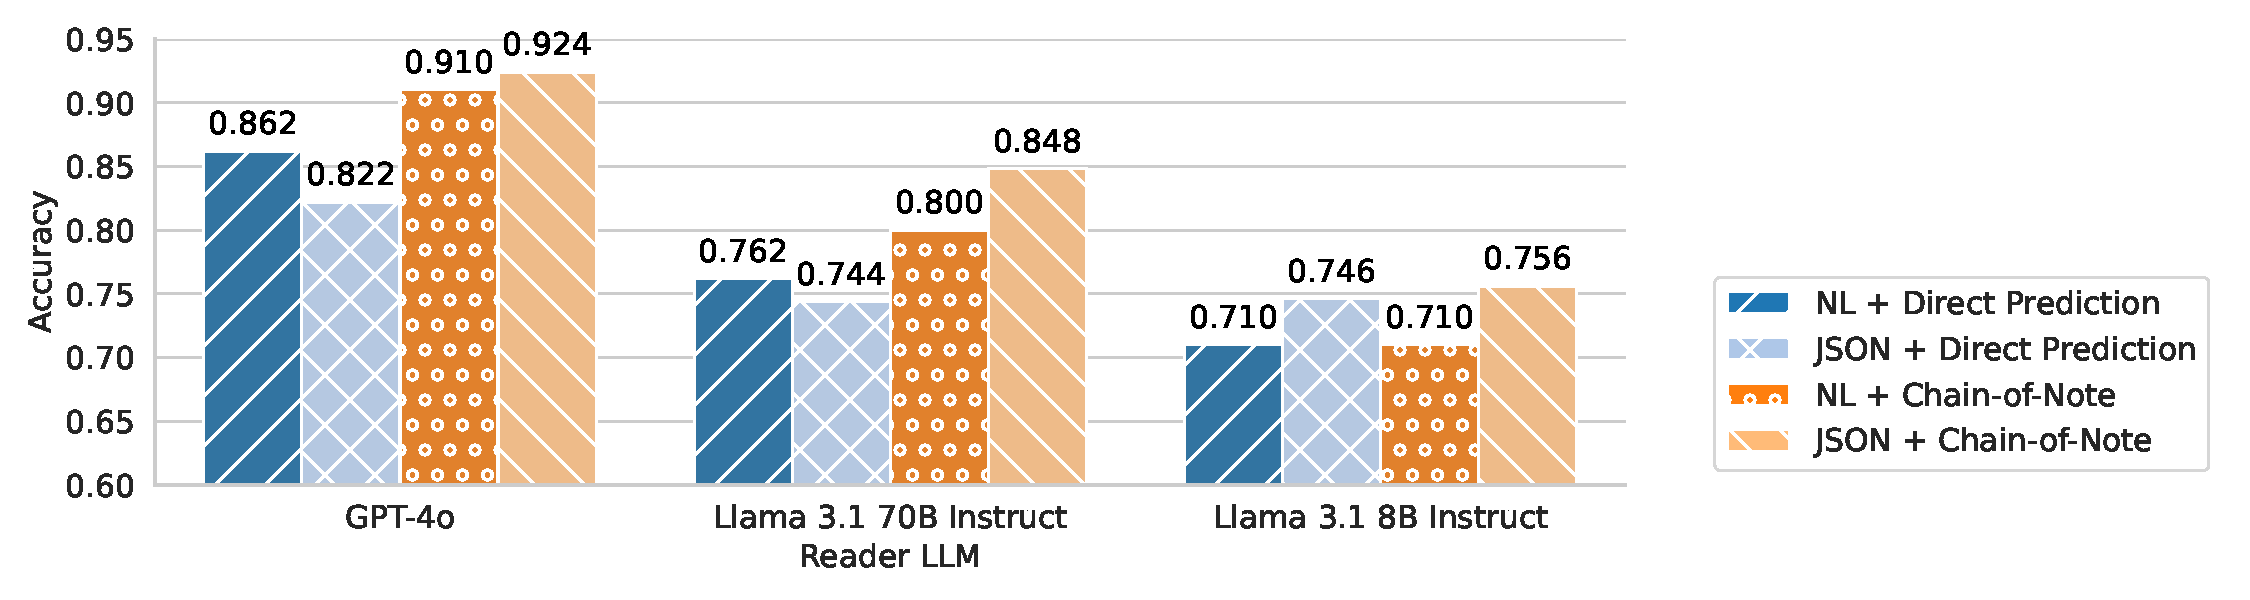
\includegraphics[width=0.9\textwidth]{figures/compare_reading_choice.pdf} 
 \vspace{-3mm}
 \caption{Question answering performance under the oracle retrieval setting. CoN with JSON format outperforms the other three parameter combinations by a large margin. {NL = Natural Language.}}
 \label{fig:main-fig-reading-design}
 \vspace{-3mm}
\end{figure}
